\chapter{METHODOLOGY}
This project aims to fine-tune the Llama-2 7B large language model for Python code generation. The methodology is structured into three distinct phases: dataset preparation, model fine-tuning, and performance evaluation.

Figure~\ref{fig:finalmodel} illustrates the system block diagram, while Figure~\ref{fig:decoder} provides a detailed view of the decoder block with the integrated QLoRA adapter.



\begin{figure}[H]
    \centering
    \includegraphics[width=0.65\linewidth]{model.jpg}
    \caption{System Block Diagram}
    \label{fig:finalmodel}
\end{figure}

\begin{figure}[H]
    \centering
    \includegraphics[width=0.85\linewidth]{decoder.jpg}
    \caption{Decoder Block Diagram with QLoRA Adapter}
    \label{fig:decoder}
\end{figure}

The architecture follows a decoder-only Transformer design. Input text is converted into embeddings and combined with positional encodings before entering a stack of 32 decoder layers (for Llama-2 7B). Within each layer, data passes through RMSNorm and a multi-head self-attention mechanism. Crucially, the QLoRA adapters are injected into the linear projections of the attention and Feed-Forward Network (FFN) blocks. This allows for task-specific parameter updates while keeping the base model's 4-bit quantized weights frozen.

\section{Dataset Description and Preparation}
Fine-tuning for Python code generation requires a high-quality dataset containing diverse programming tasks. We construct a composite dataset from multiple open-source repositories.

\subsection{Dataset Sources and Composition}
\begin{table}[H]
    \centering
    \caption{Dataset Sources and Composition}
    \begin{tabularx}{\textwidth}{|>{\bfseries}l|X|X|l|}
        \hline
        \textbf{Dataset} & \textbf{Size} & \textbf{Content \& Reason} & \textbf{License} \\ \hline
        FlyTech Python & $\sim$42,000 pairs & Python scripts with structured tasks and docstrings. & MIT \\ \hline
        Alpaca-18k & $\sim$18,000 pairs & Instruction prompts for prompt diversity. & CC BY-NC \\ \hline
        LeetCode & 200--300 & Competitive tasks for functional testing. & Fair use \\ \hline
    \end{tabularx}
    \label{tbl:datasets}
\end{table}

\subsection{Dataset Processing Pipeline}
The collected data undergoes a rigorous preprocessing pipeline:
\begin{itemize}
    \item \textbf{Duplicate Removal:} Eliminating identical instruction–code pairs to prevent overfitting.
    \item \textbf{Syntactic Filtering:} Discarding incomplete or syntactically incorrect Python code using AST parsing.
    \item \textbf{Chain-of-Thought (CoT) Enrichment:} Adding step-by-step reasoning to help the model learn logical structure.
    \item \textbf{Normalization:} Standardizing indentation (PEP 8) and naming conventions.
\end{itemize}



\begin{table}[H]
    \centering
    \caption{Final Expected Dataset Size}
    \begin{tabular}{l r}
        \textbf{Source} & \textbf{Count} \\ \hline
        FlyTech & $\sim$40,000 \\
        Alpaca & $\sim$17,000 \\ \hline
        \textbf{Total Usable Examples} & \textbf{$\sim$57,000} \\
    \end{tabular}
\end{table}

\subsection{Instruction Formatting and Tokenization}
Each example is formatted into an instruction-style structure. For example:
\begin{quote}
\texttt{Instruction:} Write a Python code for printing whether a given number is Armstrong.\\
\texttt{Chain of thought:} [Logical steps...]\\
\texttt{Response:} [Python Code Block]
\end{quote}

\section{Model Fine-Tuning}
The model utilizes the instruction-tuning paradigm. Given a prompt $x$, the model predicts the target token sequence $y$ by maximizing the likelihood:
\begin{equation}\label{eq:loss}
\mathcal{L} = -\sum_{t=1}^{T} \log P_{\theta} (y_{t} \mid y_{<t}, x)
\end{equation}

\subsection{QLoRA for Efficient Training}
QLoRA achieves efficiency by freezing the 4-bit quantized base weights and optimizing only the low-rank adapter matrices. This reduces the VRAM requirement to approximately 16GB, fitting within the constraints of an NVIDIA RTX 3060 or Google Colab T4.

\begin{figure}[H]
    \centering
    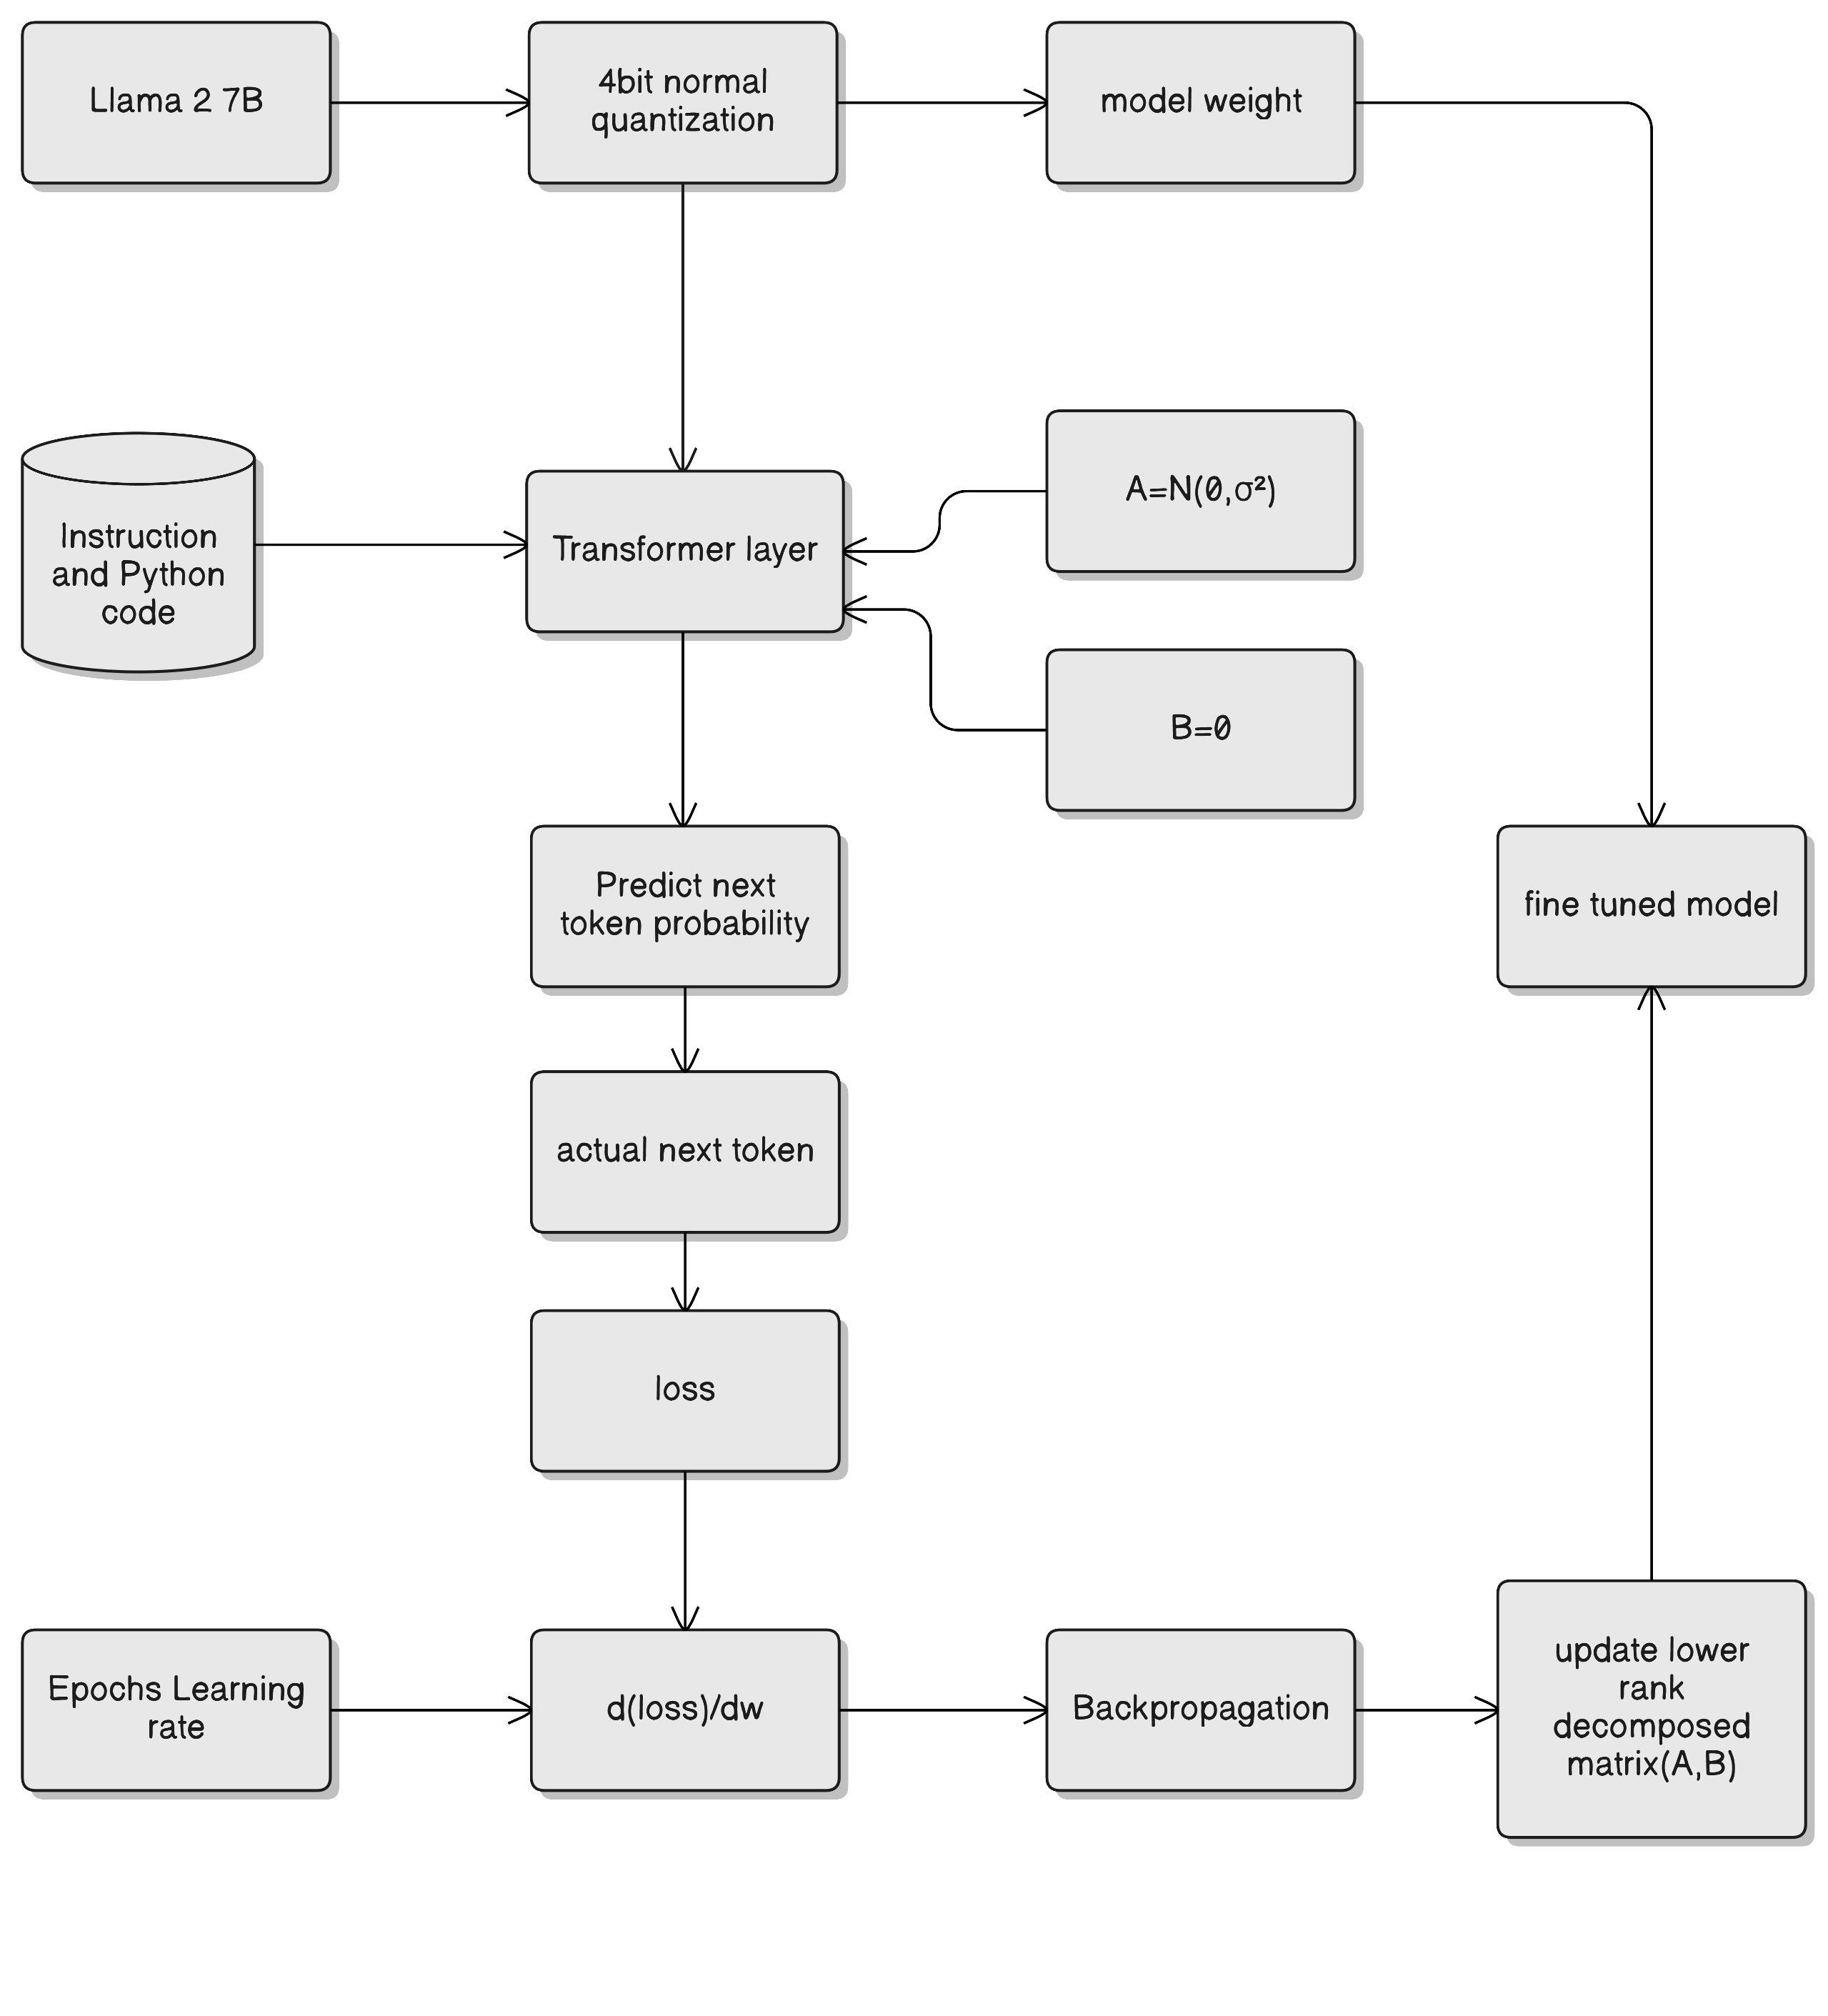
\includegraphics[width=1\linewidth]{flowdiagram.png} 
    \caption{Base Model Fine-tuning with QLoRA Adapter Layers}
    \label{fig:qlora_flow}
\end{figure}

\section{Evaluation Metrics}
Evaluation is split into functional correctness and similarity-based metrics.

\subsection{Functional Correctness}
Generated solutions are executed in a secure Docker sandbox and classified as:
\begin{itemize}
    \item \textbf{Right:} Passes all test cases.
    \item \textbf{Partial:} Passes some test cases.
    \item \textbf{Wrong:} Fails output or crashes.
\end{itemize}

\subsection{Automatic Similarity Metrics}
We utilize BLEU and CodeBLEU for quantitative assessment. CodeBLEU integrates structural information via Abstract Syntax Trees (AST) and data-flow:
\begin{equation}
\text{CodeBLEU} = \alpha \cdot \text{BLEU} + \beta \cdot \text{AST} + \gamma \cdot \text{DFScore} + \delta \cdot \text{SemanticScore}
\end{equation}
where $\alpha, \beta, \gamma, \delta$ are weighted parameters.